\newcommand{\fwb}{2.45cm}  % width
\newcommand{\fwh}{1.8cm}     % height
\begin{figure}[t]
\centering
\begin{tabular}{C{\fwb}C{\fwb}C{\fwb}}
%kernel & draws from GP & GP posterior \\
\rotatebox{90}{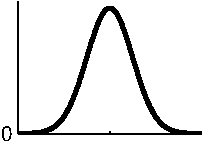
\includegraphics[width=\fwh,height=\fwb]{../figures/structure_examples/se_kernel}} &  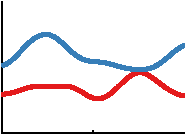
\includegraphics[width=\fwb,height=\fwh]{../figures/structure_examples/se_kernel_draws} & 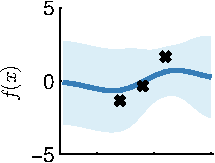
\includegraphics[width=\fwb,height=\fwh]{../figures/structure_examples/se_kernel_post} \\
squared-exp & locally smooth & little extrapolation \\ \midrule
\rotatebox{90}{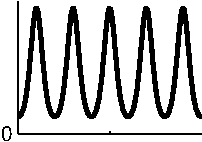
\includegraphics[width=\fwh,height=\fwb]{../figures/structure_examples/per_kernel}} &  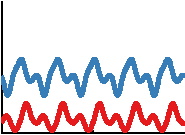
\includegraphics[width=\fwb,height=\fwh]{../figures/structure_examples/per_kernel_draws} & 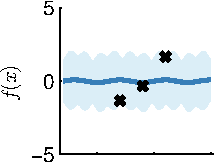
\includegraphics[width=\fwb,height=\fwh]{../figures/structure_examples/per_kernel_post} \\
periodic & repeated structure & long-range dependency \\ \midrule
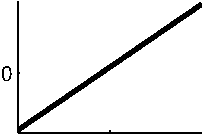
\includegraphics[width=\fwb,height=\fwh]{../figures/structure_examples/lin_kernel} &  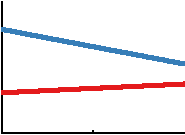
\includegraphics[width=\fwb,height=\fwh]{../figures/structure_examples/lin_kernel_draws} & 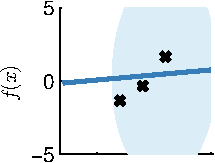
\includegraphics[width=\fwb,height=\fwh]{../figures/structure_examples/lin_kernel_post} \\
linear & linear & linear \\ \midrule
\rotatebox{90}{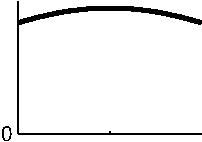
\includegraphics[width=\fwh,height=\fwb]{../figures/structure_examples/longse_kernel}} &  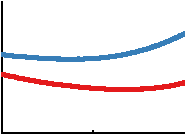
\includegraphics[width=\fwb,height=\fwh]{../figures/structure_examples/longse_kernel_draws} & 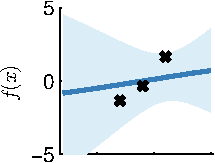
\includegraphics[width=\fwb,height=\fwh]{../figures/structure_examples/longse_kernel_post} \\
long-lengthscale squared-exp & slowly changing & moderate extrapolation
\end{tabular}
\caption{ Properties of basic kernels.  The x-axis has the same scale for all plots.  The leftmost column shows the kernel function, the central column shows draws from a zero-mean GP with that kernel, and the right-most column shows a GP posterior after conditioning on two datapoints.
\TBD{RBG: Do we need this figure?  It's pretty standard stuff, and it's largely subsumed by Figure 2.}}
\label{fig:basic_kernels}
\end{figure}
